\begin{frame}{Bias and Variance}

\begin{itemize}
    \item What if $Y$ has a non-linear response?
\end{itemize}

\begin{center}
    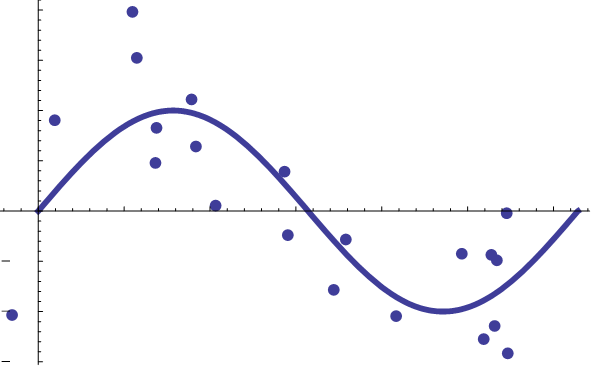
\includegraphics[width=0.65\linewidth]{images/linear-regression/linear-regression-13.png}
\end{center}

\vspace{-0.3cm}
\begin{itemize}
    \item Can we still use a linear model?
\end{itemize}

\end{frame}


\begin{frame}{What is Bias and Variance?}

\begin{columns}
    \column{0.5\textwidth}
    \begin{center}
        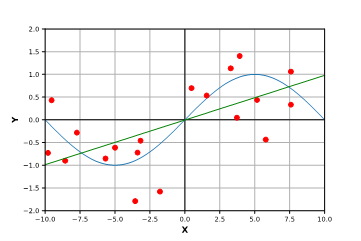
\includegraphics[width=0.95\linewidth]{images/linear-regression/linear-regression-14.png} \\
        $\{1, x\}$
    \end{center}
    
    \column{0.5\textwidth}
    \begin{center}
        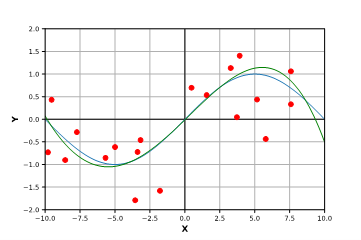
\includegraphics[width=0.95\linewidth]{images/linear-regression/linear-regression-15.png} \\
        $\{1, x, x^{[2]}, x^{[3]}, x^{[4]}\}$
    \end{center}
\end{columns}

\vspace{0.2cm}

\begin{columns}
    \column{0.5\textwidth}
    \begin{center}
        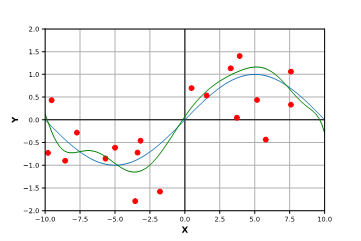
\includegraphics[width=0.95\linewidth]{images/linear-regression/linear-regression-16.png} \\
        $\{1, x, x^{[2]}, \dots, x^{[10]}\}$
    \end{center}
    
    \column{0.5\textwidth}
    \begin{center}
        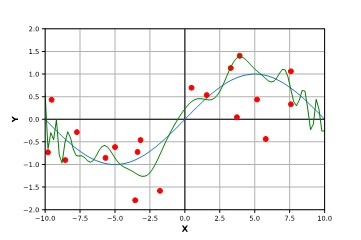
\includegraphics[width=0.95\linewidth]{images/linear-regression/linear-regression-17.png} \\
        $\{1, x, x^{[2]}, \dots, x^{[100]}\}$
    \end{center}
\end{columns}

\end{frame}


\begin{frame}{Real Bad Overfit?}
    \centering
    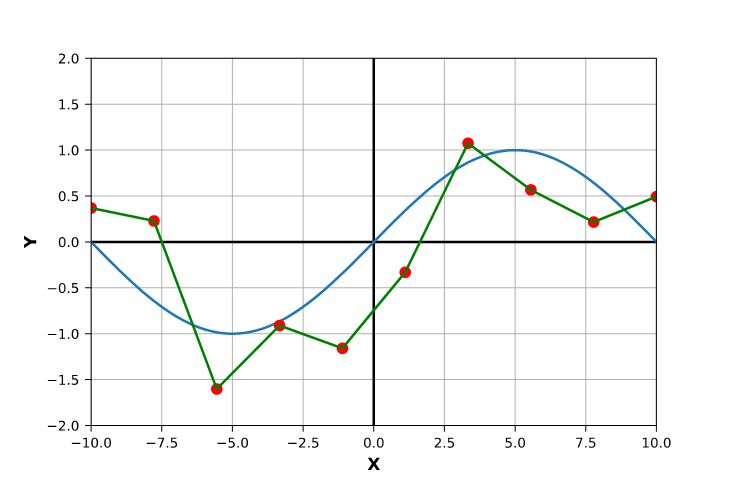
\includegraphics[width=0.9\linewidth]{images/linear-regression/linear-regression-18.png}
\end{frame}


\begin{frame}{Bias-Variance Tradeoff}
\begin{itemize}
    \item So far, we have minimized the error (loss) with respect to \textbf{training data}
    \begin{itemize}
        \item Low training error does not imply good expected performance: \textbf{over-fitting}
    \end{itemize}
    \item We would like to reason about the \textbf{expected loss (Prediction Risk)} over:
    \begin{itemize}
        \item Training Data: $\{(y_1, x_1), \ldots, (y_n, x_n)\}$
        \item Test point: $(y_*, x_*)$
    \end{itemize}
    \item We will decompose the expected loss into:
\end{itemize}

\[
\mathbb{E}_{D,(y_*, x_*)} \left[ \left( y_* - f(x_* \mid D) \right)^2 \right]
= \text{Noise} + \text{Bias}^2 + \text{Variance}
\]
\end{frame}


\begin{frame}{Bias Variance Plot}
    \begin{figure}
        \centering
        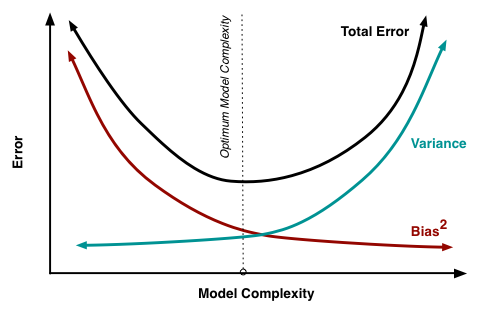
\includegraphics[width=0.9\linewidth]{images/linear-regression/linear-regression-19.png}
    \end{figure}
    \vspace{-1em}
    \footnotesize{Image from \url{http://scott.fortmann-roe.com/docs/BiasVariance.html}}
\end{frame}
